\chapter{Working Strategy of gr-cdma}
In this chapter, we will discuss the working strategy of gr-cdma, the principle of each main block.
Mathematic models and analyses are involved to describe the situation.

\section{The diagram of The Tx \& Rx}
Here are the digrams for Tx and Rx. 
\begin{figure}[!ht]
	\centering
	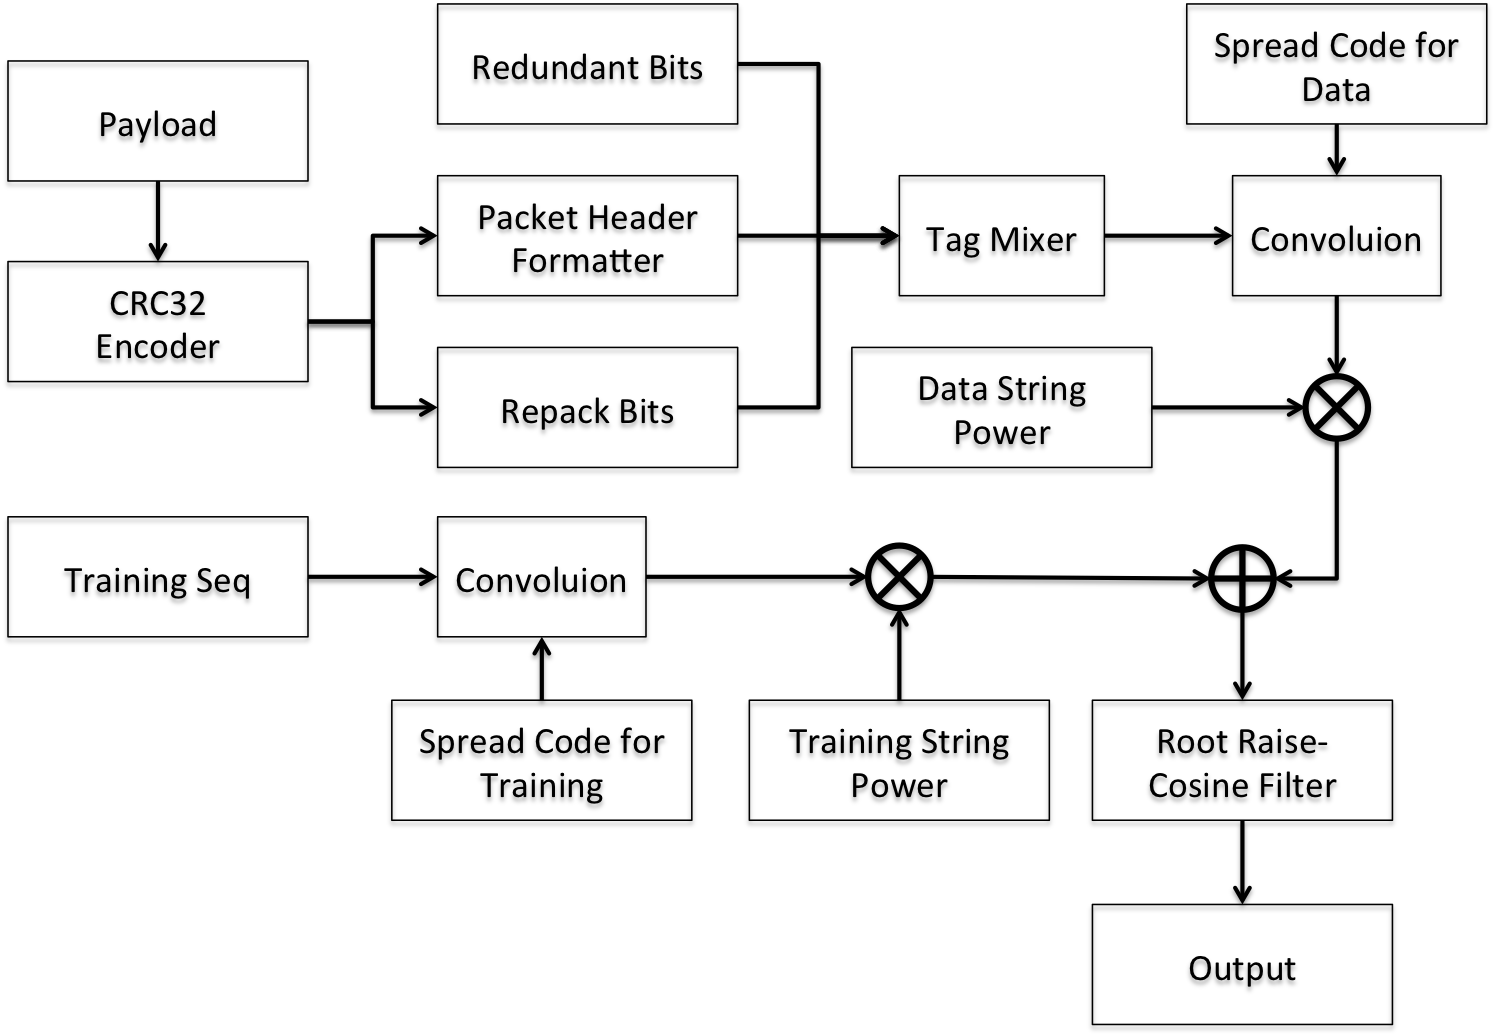
\includegraphics[width = 5 in]{figure/tx-diagram.png}
	\caption{Diagram for Tx}
	\label{fig:diagram for Tx}
\end{figure}
\begin{figure}[!ht]
	\centering
	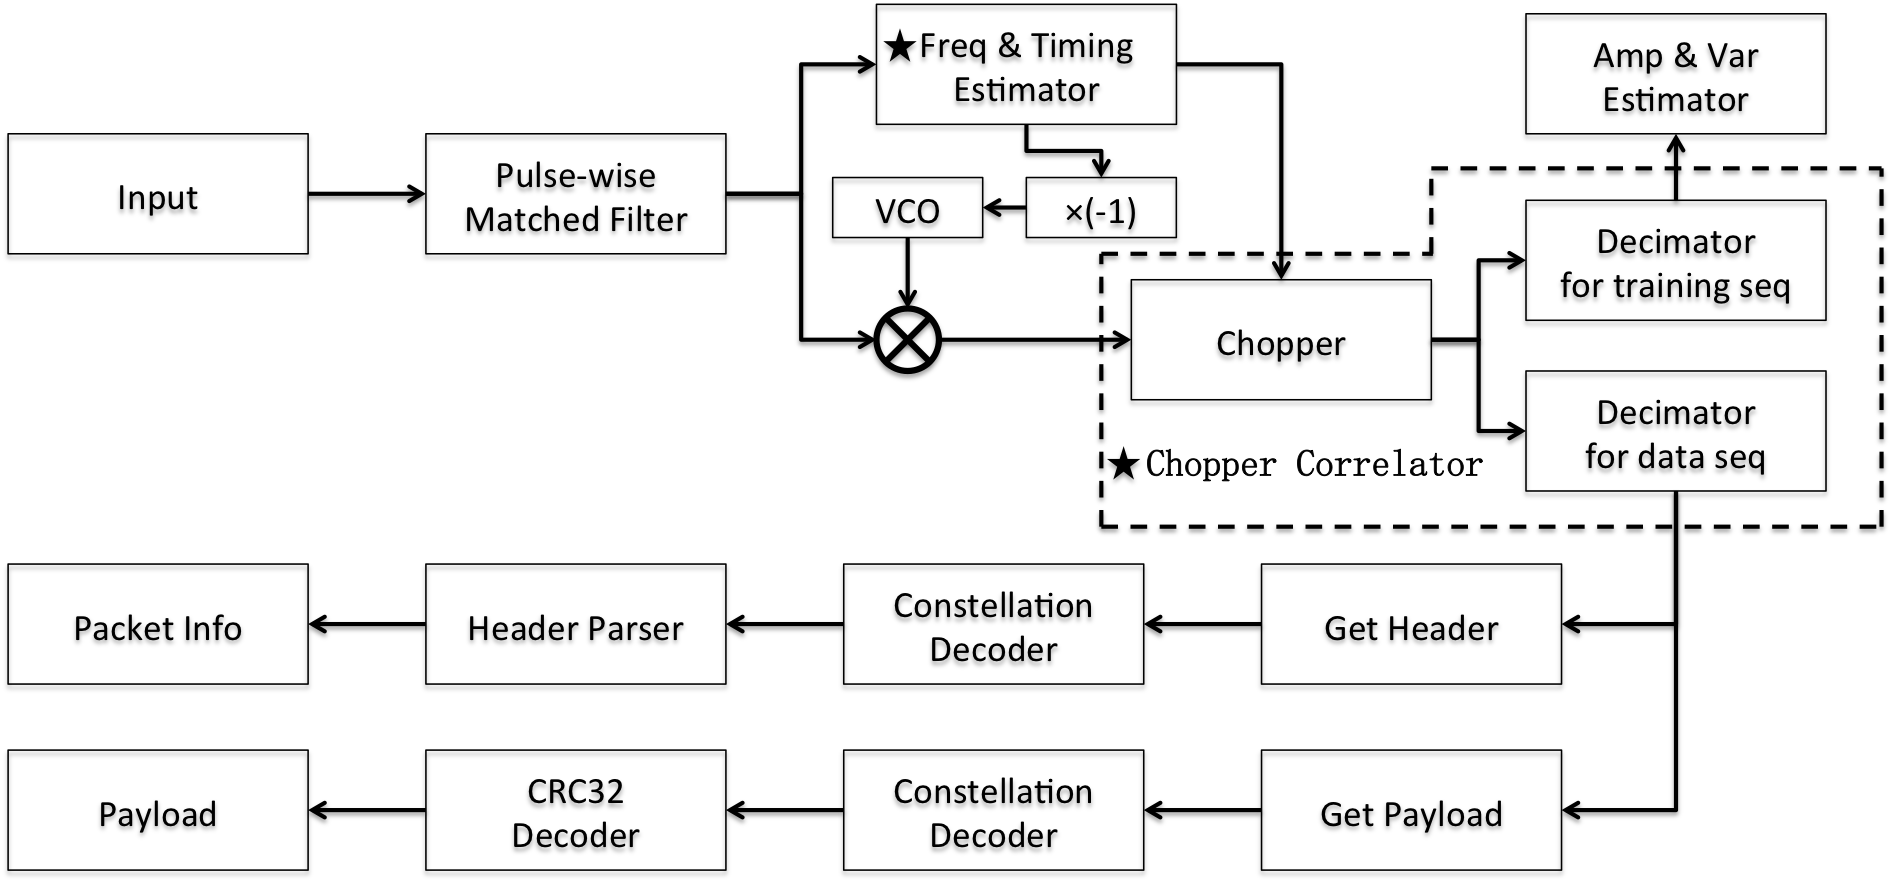
\includegraphics[width = 5in]{figure/rx-diagram.png}
	\caption{Diagram for Rx}
	\label{fig:diagram for Rx}
\end{figure}

From fig \ref{fig:diagram for Tx} and fig \ref{fig:diagram for Rx}, you may find that the system is a little bit more complicated than you thought. And also, the receiver is bigger than the transmitter. In fact, it is for the reason that the receiver will deal with no only the decoding part, but also the synchronization problem. which is actually the most difficult part for this system.

\section{Transmitter} % (fold)
\label{sec:transmitter}
The duty for transmitter is to package the payload or the input data, build the packet structure, generate the training sequence, modify the power for each section and form the waveform. Similar to other CDMA system, one of the essential part of the system is about the spreading code. The quality of the spreading code will affect greatly about the performance of synchronization parts. Intuitively, we would like to use codes like m-sequences and gold sequence, which has high auto-correlation and flat cross-correlation value.

\begin{figure}
	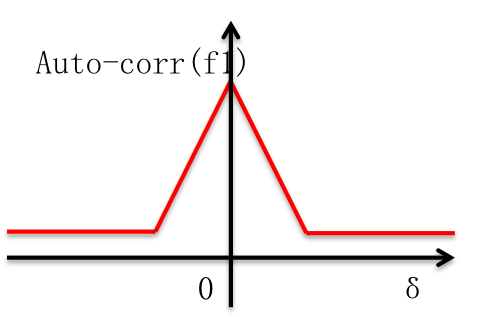
\includegraphics[width = 3in]{figure/bad_correlation.png}
	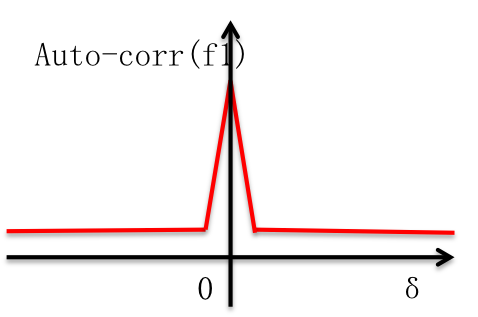
\includegraphics[width = 3in]{figure/good_correlation.png}
\end{figure}

% section transmitter (end)